\documentclass[landscape]{foils}
\usepackage[pdftex]{color}
\usepackage[pdftex]{graphicx}
\usepackage{eso-pic}
\usepackage[top=2cm, bottom=2cm, outer=0cm, inner=0cm]{geometry}
\usepackage{listings}
\usepackage{amsmath}
\usepackage[pdftex,colorlinks=false,urlbordercolor={0.667 0.110 0.094}]{hyperref}


\DeclareMathOperator{\sign}{sign}

% colors
\definecolor{DarkRed}{rgb}{0.5,0.0,0.0}
\definecolor{DarkBlue}{rgb}{0.0,0.0,0.35}
\definecolor{DarkGreen}{rgb}{0.0,0.6,0.00}
\definecolor{Orange}{rgb}{0.70,0.30,0.0}
\definecolor{Magenta}{rgb}{0.8,0.0,0.8}
\definecolor{DarkGray}{rgb}{0.3,0.3,0.3}
\def\red{\color{red}} 
\def\darkred{\color{DarkRed}} 
\def\blue{\color{DarkBlue}} 
\def\green{\color{DarkGreen}} 
\def\orange{\color{Orange}}
\def\magenta{\color{Magenta}}
\def\black{\color{black}}
\def\gray{\color{DarkGray}}

% sizes, footer and headers
\textwidth = 26truecm
\textheight = 18truecm
\topmargin =-2 cm
\oddsidemargin -1.5cm
\rightfooter{}
\MyLogo{\darkred {\bf QE-2019}: Summer School on Advanced Materials
  and Molecular Modelling}
%
\def\indent{\hspace*{1cm}}
\def\prompt{\texttt{\$~}}
\def\exec#1{\indent\prompt\code{#1}}
\def\codeline#1{\indent\code{#1}}
\parindent 0pt

% alias for slides header
\def\Head#1{\foilhead{\red #1 \vskip -1cm} \medskip\hrule\medskip}
\def\head#1{\foilhead{\red #1 \vskip -1cm}}

% aliases for codes, files, namelists, etc.
\def\codecolor{\green}
\def\cardcolor{\orange}
\def\code#1{\texttt{\codecolor #1}}
\def\prog#1{\texttt{\red #1}}
\def\var#1{\texttt{\red #1}}
\def\file#1{\texttt{\green #1}}
\def\cmd#1{\texttt{\green #1}}
\def\nml#1{\texttt{\magenta #1}}
\def\card#1{\texttt{\cardcolor #1}}
\def\flag#1{\texttt{\green #1}}

% aliases for math
\def\vr{\ensuremath{\bm{r}}}
\def\vR{\ensuremath{\bm{R}}}
\def\vk{\ensuremath{\bm{k}}}
\def\vtau{\ensuremath{\bm{\tau}}}

\def\pwtk{\href{http://pwtk.ijs.si}{PWTK}}

\begin{document}
\AddToShipoutPictureBG*{
\includegraphics[width=\paperwidth,height=\paperheight]{figs/qe2021-background-4x3.png}}

\blue
%
\includegraphics[width=1.0\textwidth]{figs/QE2019-logo.pdf}
~\\
\vspace*{4cm}
\MyLogo{~}
\vspace{3em}
\begin{center}
  {\burgundy\LARGE\bf QE-2021: Hands-on session -- Day-2}\\[2em]
  {\burgundy\LARGE (Convergence-tests calculations)}
  ~\\[1.5em]
  \large Anton Kokalj, Pietro Delugas, Paolo Giannozzi, \\
  Matic Pober\v{z}nik, Cristiano Malica, Subrahmanyam Sappati, Lei Qiao
\end{center}

%%%%%%%%%%%%%%%%%%%%%%%%%%%%%%%%%%%%%%%%%%%%%%%%%%%%%%%%%%%%% 
\Head{QE-2021: Hands-on session -- Day-2}
\MyLogo{\burgundy {\bf QE-2021}: MaX School on Advanced Materials and Molecular Modelling}
\rightheader{\hspace{-0.8cm}
\includegraphics[width=4.5cm]{figs/QE.png}}
Topics of Day-2 hands-on session:
\begin{enumerate}
\item How to make basic convergence tests (\file{example1.Si/})
\item How to deal with metals (\file{example2.Al/})
\item How to deal with ultrasoft pseudopotentials and with spin polarization
  (\file{example3.Fe/})
\end{enumerate}

To get the latest version of the exercises, move to \file{Day-2/} directory and execute:\\[0.5em]
\exec{git pull}

{\bf Beware:} if you changed some input files in \file{Day-1/} then
\file{git pull} will fail and you will need to do:\\[0.5em]
\exec{git stash}\\
\exec{git pull}\\
\exec{git stash apply}\\

    
%%%%%%%%%%%%%%%%%%%%%%%%%%%%%%%%%%%%%%%%%%%%%%%%%%%%%%%%%%%%% 
\head{1. Bulk system: Silicon}
\rightfooter{Example: \file{Day-2/example1.Si/}}
%
Self-consistent calculation (and a series of tests) for Silicon in the
diamond structure:
\begin{itemize}
\item move to \file{Day-2/example1.Si/} directory
\item look at the input file \file{pw.si.scf.in}. It is composed of three
``namelists'' \nml{\&CONTROL} (note that \var{calculation = 'scf'}
is the default value), \nml{\&SYSTEM}, \nml{\&ELECTRONS}, followed 
by three ``cards'' \card{ATOMIC\_SPECIES}, \card{ATOMIC\_POSITIONS},
\card{K\_POINTS}
\item in the \nml{\&CONTROL} namelist notice the following two
  variables (they are commented):
  \begin{itemize}
  \item \var{outdir}: temporary directory for large files.
    Must be writable, will be created if not existent.
    You may set environment variable \var{ESPRESSO\_TMPDIR} instead.\\[-0.5em]
    
  \item \var{pseudo\_dir}: directory where pseudopotential (PP)
    files are kept.
    It must exist, be readable, and contain the required PP file
    (in this example, \file{Si.pz-vbc.UPF} for Silicon).
    You may set environment variable \var{ESPRESSO\_PSEUDO}
    instead.
  \end{itemize}
\end{itemize}

(note that for the hands-on exercises we rely on
\var{ESPRESSO\_TMPDIR} and \var{ESPRESSO\_PSEUDO} environmental
variables, hence we don't need to set \var{outdir} and
\var{pseudo\_dir} variables)

%%%%%%%%%%%%%%%%%%%%%%%%%%%%%%%%%%%%%%%%%%%%%%%%%%%%%%%%%%%%%
\head{\burgundy Providing atomic structure in input}
\begin{itemize}
\item[]
\parbox{15cm}{How is the crystal structure defined? This is a very
simple case: the diamond lattice is an fcc (face-centered cubic) lattice
with two atoms per unit cell. You need to specify:}\hskip 1cm
\parbox{10cm}{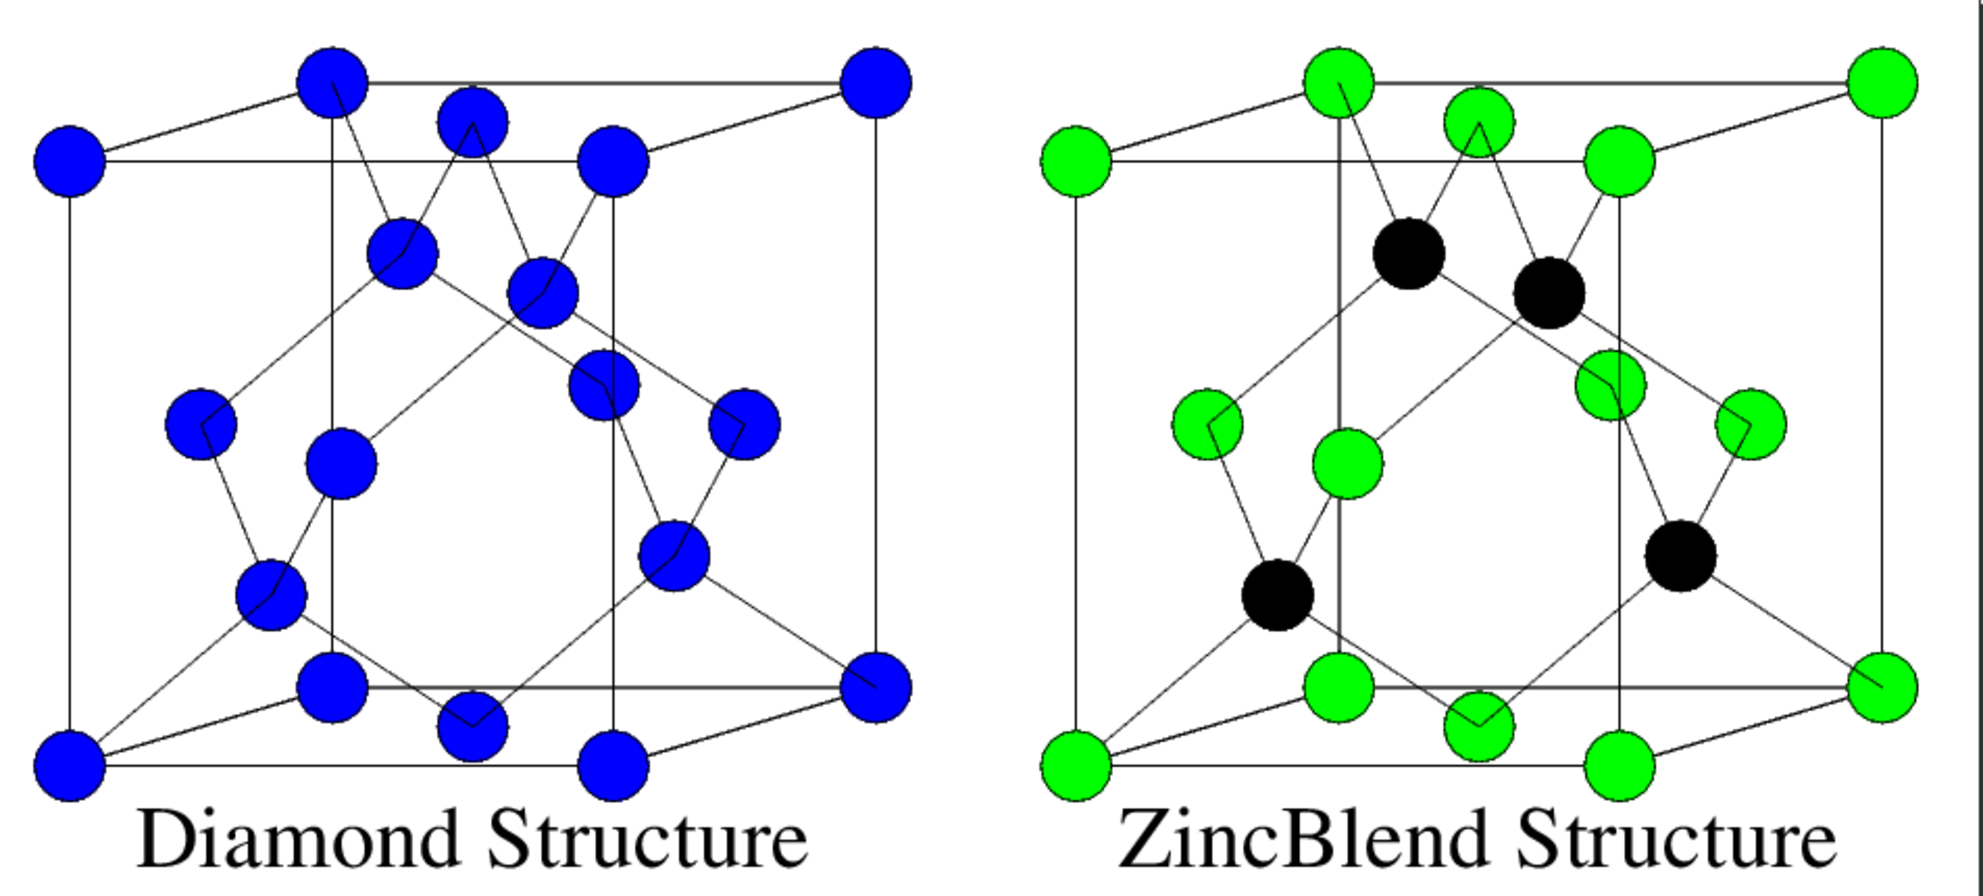
\includegraphics[width=8cm]{figs/Dia-ZB.pdf}}
\begin{itemize}
\item  What is the Bravais lattice?\\
  {\gray \var{ibrav=2}, meaning fcc lattice}
\item  How many and which parameters are needed to completely 
  define Bravais lattice?\\
  {\gray just one: \var{celldm(1)=10.2}, lattice parameter $a$ in a.u.}
\item  How many atoms there are in the unit cell?\\
{\gray  \var{nat=2}: two atoms}
\item  How many different atomic species are present?\\
{\gray  \var{ntyp=1}: one species}
\item  Which ones, described by which pseudopotential? \\
{\gray  See card \card{ATOMIC\_SPECIES}}
\item  Where the atoms are located in the unit cell?\\
{\gray  See card \card{ATOMIC\_POSITIONS}: here, in Cartesian axes,
       in units of $a$ (``\flag{alat}'')}
\end{itemize}
\item[]Notice that there are several alternative methods to specify an atomic structure!
\end{itemize}

%%%%%%%%%%%%%%%%%%%%%%%%%%%%%%%%%%%%%%%%%%%%%%%%%%%%%%%%%%%%% 
\head{Brillouin zone (BZ) sampling}

{\bf k-points} are described in the \card{K\_POINTS} card. One has to choose

\begin{itemize}
\item  Whether to provide a list of k-points or a uniform grid\\

\item  If a list is chosen: provide a list of k-points {\em in the Irreducible
BZ} and corresponding symmetry weights; the latter do not need to add 
up to 1, they are normalized by the code\\[1em]
{\bf Frequently Asked Question:} where do I find special k-points 
and their weights?\\
{\gray Answer: 1) in papers, 2) use an auxiliary code \prog{kpoints.x}, 
  3) {\bf use uniform grids}}

\item If a uniform grid is chosen: specify Monkhorst-Pack parameters
  {\small ({\sl Phys. Rev. B} {\bf 13}, 5188 (1976))} and offsets
  along the three directions {\gray (uniform k-point grids are covered
    in more detail in section 1.2 below)}.
\end{itemize}

%%%%%%%%%%%%%%%%%%%%%%%%%%%%%%%%%%%%%%%%%%%%%%%%%%%%%%%%%%%%%
\head{Running the pw.x code}
For serial (single processor) execution you can use\\[0.5em]
\exec{pw.x -in pw.si.scf.in > pw.si.scf.out}\\[0.5em]
{\small (note: input redirection \code{pw.x < pw.si.scf.in} works but it
  is not recommended on parallel machines)}

\vspace{-1em}
Look at the directory specified by \var{outdir} (in our case
\var{\$ESPRESSO\_TMPDIR}) and its content:\\[0.5em] 
\exec{ls \$ESPRESSO\_TMPDIR}\\
\codeline{silicon.save  silicon.xml}\\[0.3em]
{\small\gray (to see only these files, you may need to use
\code{ls \$ESPRESSO\_TMPDIR/silicon.*})}\\

The directory contains a data directory (\file{silicon.save/}) with
binary data files for further processing and an XML file
(\file{silicon.xml}) with general information on the run.  The name of
the various files is determined by the value of the \var{prefix}
variable and by their content.

{\burgundy\em Do not run two instances of \prog{pw.x} that access the same
  \texttt{outdir} with the same \texttt{prefix}!} Unpredictable
behavior may follow (the directory is used for temporary files as
well).  In case of trouble, clean \var{outdir}.

%%%%%%%%%%%%%%%%%%%%%%%%%%%%%%%%%%%%%%%%%%%%%%%%%%%%%%%%%%%%%
\head{Running the pw.x code (II)}
Examine output file \file{pw.si.scf.out}, look how self-consistency proceeds:
{\codecolor
\begin{verbatim}
$ grep -e "total energy" -e estimated pw.si.scf.out
     total energy              =     -15.79103344 Ry
     estimated scf accuracy    <       0.06376674 Ry
     total energy              =     -15.79409289 Ry
     estimated scf accuracy    <       0.00230109 Ry
     total energy              =     -15.79447822 Ry
     estimated scf accuracy    <       0.00006291 Ry
     total energy              =     -15.79449510 Ry
     estimated scf accuracy    <       0.00000448 Ry
!    total energy              =     -15.79449593 Ry
     estimated scf accuracy    <       0.00000005 Ry
     The total energy is the sum of the following terms:
\end{verbatim}
}
Notice that there are 8 electrons in the cell: 2 (pseudo-)atoms/cell
with 4 electrons. The system is a non-magnetic insulator, so just the 
lowest 4 (= 8/2) valence bands (Kohn-Sham states) are computed.

%%%%%%%%%%%%%%%%%%%%%%%%%%%%%%%%%%%%%%%%%%%%%%%%%%%%%%%%%%%%% 
\head{1. Convergence tests for Si bulk}

Convergence tests for Si bulk consist of the following steps:
\begin{enumerate}
\item convergence with respect to basis-set, i.e., kinetic energy
  cutoff (variable \var{ecutwfc})
\item convergence with respect to k-points (card \var{K\_POINTS})

\item with converged \var{ecutwfc} and k-points, determine the lattice
  parameter of Si bulk

\item Bonus: with converged parameters (\var{ecutwfc}, k-points, and
  lattice parameter), calculate a band structure of Si-bulk
\end{enumerate}


%%%%%%%%%%%%%%%%%%%%%%%%%%%%%%%%%%%%%%%%%%%%%%%%%%%%%%%%%%%%% 
\head{1.1 Convergence w.r.t.\@{} the kinetic energy cutoff}
%
\rightheader{\hspace{-0.8cm}
\includegraphics[width=3.4cm]{figs/QE.png}}

The kinetic energy cutoff \var{ecutwfc} (in Ry) determines the size of
the Plane-Wave (PW) basis set used to expand wave-functions (i.e.
Kohn-Sham orbitals) \\
{\small\gray (the default for the charge density is
  \var{ecutrho=4*ecutwfc}, which is OK for norm-conserving PPs)}

\begin{itemize}
\item A manual test of convergence w.r.t.\@{} kinetic energy cutoff entails the
following tasks\\({\bf BEWARE: we will {\burgundy not} do it manually!})
\begin{enumerate}
\item change \var{ecutwfc} in the \file{pw.si.scf.in} input to, e.g.,
  16, 20, 24, 28, 32 Ry
\item for each value of \var{ecutwfc}, run \prog{pw.x} and collect the
  final total energy
\item collect the data in a file, say \file{si.etot\_vs\_ecut}
  (i.e. each line should contain two values: \var{ecutwfc} and ``total-energy'')
\item plot the energies collected in \file{si.etot\_vs\_ecut} using your preferred
  plotting program, for instance:\\[0.5em]
  \exec{gnuplot}\\
  \codeline{gnuplot> plot 'si.etot\_vs\_ecut' with lines}
\end{enumerate}
\item because such a manual procedure is very cumbersome we use
  scripts instead
\end{itemize}

%%%%%%%%%%%%%%%%%%%%%%%%%%%%%%%%%%%%%%%%%%%%%%%%%%%%%%%%%%%%% 
\head{\burgundy 1.1 Convergence w.r.t.\@{} kinetic energy cutoff (II)}
\rightheader{\hspace{-0.8cm}
\includegraphics[width=3.4cm]{figs/QE.png}}
%
To make convergence tests easier and faster, scripts are commonly
used. To this end, Unix shell-scripts have been traditionally used,
yet there are other more "fancy" alternatives, e.g., \pwtk\
scripts.\vspace{-1em}
{\small
  \begin{itemize}
  \item A Unix shell-script is located in
    \file{ex1.ecutwfc.classic/} sub-directory (file: \file{ecutwfc.sh})
  \item A PWTK script is located in \file{ex1.ecutwfc/} sub-directory
    (file: \file{ecutwfc.pwtk})
  \end{itemize}  
}
\vspace{0.5cm}
\centerline{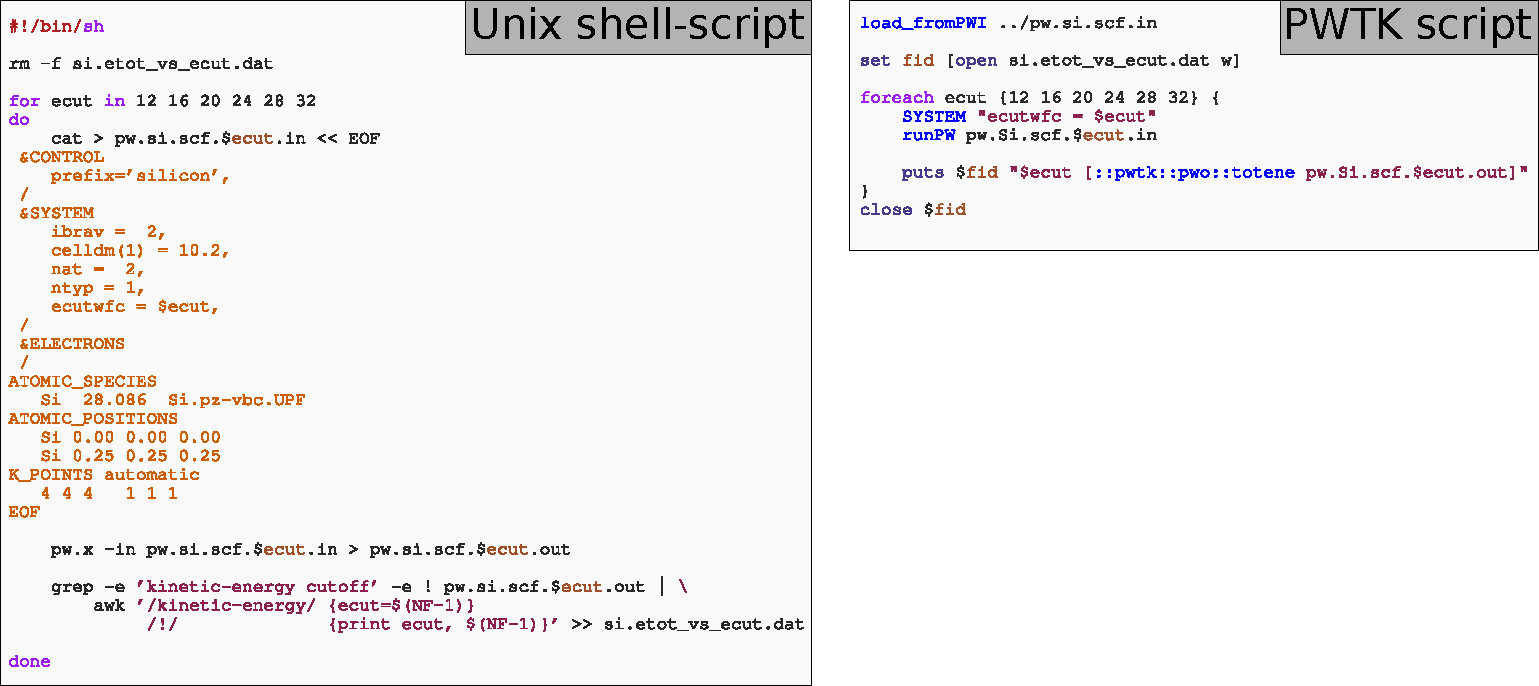
\includegraphics[width=1.0\textwidth]{figs/sh-vs-pwtk.pdf}}

%%%%%%%%%%%%%%%%%%%%%%%%%%%%%%%%%%%%%%%%%%%%%%%%%%%%%%%%%%%%%
%\head{\burgundy 101 of PWTK scripting}
\head{\burgundy PWTK scripting: basics}
\rightheader{
\includegraphics[width=2.5cm]{figs/pwtk.png}}
\rightfooter{}
The basic philosophy is to {\bf keep the syntax close to original input syntax}!\\[1.5em]
\centerline{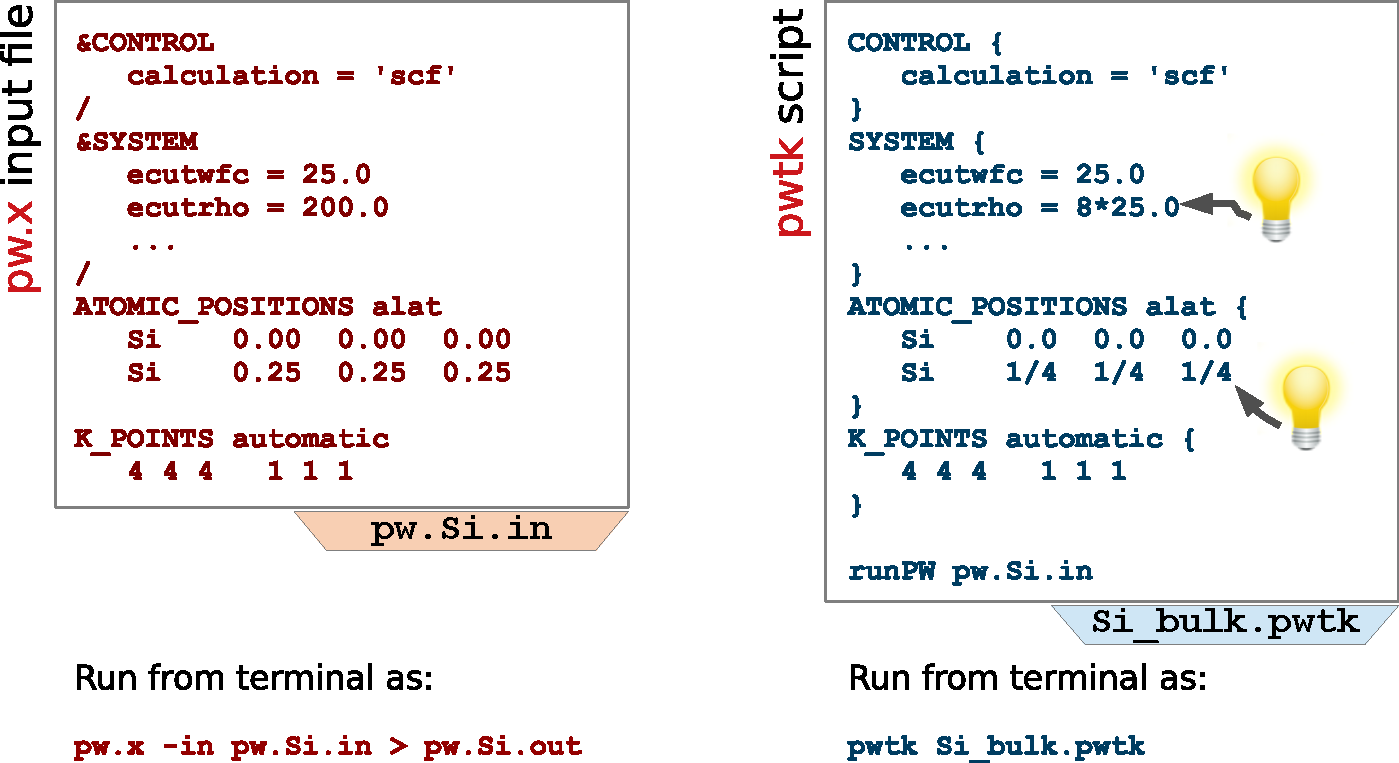
\includegraphics[width=1.0\textwidth]{figs/pwtk-syntax.pdf}}

%%%%%%%%%%%%%%%%%%%%%%%%%%%%%%%%%%%%%%%%%%%%%%%%%%%%%%%%%%%%% 
%\head{\burgundy 101 of PWTK scripting}
\head{\burgundy PWTK scripting: basics}
\vspace{-1em}
\begin{itemize}
\item \pwtk\ scripts are basically Tcl-scripts, hence they use Tcl-syntax

  \vspace{-0.5em}
\item namelists and cards have the same names as in QE (with a few
  exceptions), but they are all written in {\bf upper-case}. Their
  content is encapsulated in curly braces:\\[0.5em]
  {\codecolor\verb+CONTROL { calculation = 'scf', outdir = '/tmp/pwscf/'}+}\\
  {\codecolor\verb+ATOMIC_POSITIONS { ... }+}

  \vspace{-0.5em}
\item instead of curly braces, one can also use double-quotes
  (\code{"..."}), e.g.:\\[0.5em]
  {\codecolor\verb+SYSTEM " celldm(1) = $a "+}

  \vspace{-0.5em}
\item the difference between curly braces \code{\{...\}} and double-quotes
  \code{"..."} is that inside double-quotes the variable \code{\$a} is
  substituted by its value, whereas inside curly braces the \code{\$a}
  is treated literally (i.e. no substitution)

  \vspace{-0.5em}
\item real numbers can be specified as mathematical
  expressions {\small (e.g. \var{ecutrho = 8*25.0})}
    
  \vspace{-0.5em}
\item indices of \var{ntyp}-type array variables, such as
  \var{starting\_magnetization(i)}, can be specified with
  atomic labels, e.g.:\\[0.5em]
  {\codecolor\verb+SYSTEM { starting_magnetization(Fe) = -0.8 }+}\\[0.5em]
  where \file{Fe} is one among atomic species defined in the \card{ATOMIC\_SPECIES} card.

  \vspace{-0.5em}  
\item PWTK scripts are case sensitive, i.e.,
  {\codecolor\verb+CONTROL { ... }+} is OK,\\
  but {\codecolor\verb+control { ... }+} is not; namelist variables
  are also case sensitive!

  \vspace{-0.5em}
\item namelist {\bf variables can be set on the fly} (we will use this
  heavily)

  \vspace{-0.5em}
\item the order of namelists and cards is not important; PWTK knows
  how to construct proper input files

  \vspace{-0.5em}
\item namelists and cards can be called many times, but there is a big
  difference how multiple calls are handled for namelists and cards:
  {\bf cards} are handled in {\bf overwrite mode}, whereas {\bf
    namelists} are handled in a {\it kind of} {\bf
    append} mode. For example, the following is OK:\\[0.5em]
  {\codecolor\verb+CONTROL { calculation = 'scf' }+}\\
  {\codecolor\verb+CONTROL { outdir = '/tmp/qe' }+}\\[0.5em]
  and is equivalent to:\\[0.5em]
  {\codecolor\verb+CONTROL { calculation = 'scf' , outdir = '/tmp/qe' }+}

  \vspace{-0.5em}
\item to unset a namelist variable, set it to an empty-value; for example
  to unset the \var{outdir} variable, use:\\[0.5em]
  {\codecolor\verb+CONTROL { outdir = }+}

\item today we will use the following \pwtk\ functions:
  \begin{itemize}
  \item \code{load\_fromPWI} -- loads input data from an existing
    \prog{pw.x} input file
    \vspace{0.2em}
  \item \code{pwo\_totene} -- returns the converged total energy
    from \prog{pw.x} output\vspace{0.2em}
  \item \code{seq} -- like the Unix \prog{seq} command (returns a
    sequence of numbers)\vspace{0.2em}
  \item \code{runPW} -- constructs \prog{pw.x} input file and runs a calculation
    \vspace{0.2em}
  \item \code{runPP} -- similar as \file{runPW} but for the \var{pp.x} program
    \vspace{0.2em}
  \item \code{runDOS} -- ... for the \var{dos.x} program
    \vspace{0.2em}
  \item \code{runPROJWFC} -- ... for the \var{projwfc.x} program
  \end{itemize}
\item PWTK web-site:\\
  \file{\url{http://pwtk.ijs.si/}} ~or~ \file{\url{http://pwtk.quantum-espresso.org/}}
  \item PWTK documentation is available at:\\
    \file{\url{http://pwtk.ijs.si/documentation.html}}
\end{itemize}



%%%%%%%%%%%%%%%%%%%%%%%%%%%%%%%%%%%%%%%%%%%%%%%%%%%%%%%%%%%%%
\head{1.1 Convergence w.r.t.\@{} the kinetic energy cutoff (III)}
\rightfooter{Example: \file{Day-2/example1.Si/ex1.ecutwfc/}}
\rightheader{}
%\rightheader{\hspace{-0.8cm}
\includegraphics[width=3.4cm]{figs/QE.png}}
% 
\begin{itemize}
\item To run the convergence test via the Unix shell-script move to
  \file{ex1.ecutwfc.classic/} sub-directory (read the
  \file{README.md} file) and execute\\[0.5em]
  \exec{./ecutwfc.sh}

\item To run the convergence test via the PWTK script move to
  \file{ex1.ecutwfc/} sub-directory (read the
  \file{README.md} file) and execute\\[0.5em]
  \exec{pwtk ecutwfc.pwtk}
\end{itemize}
\vspace{-1.5cm}
\begin{flushright}
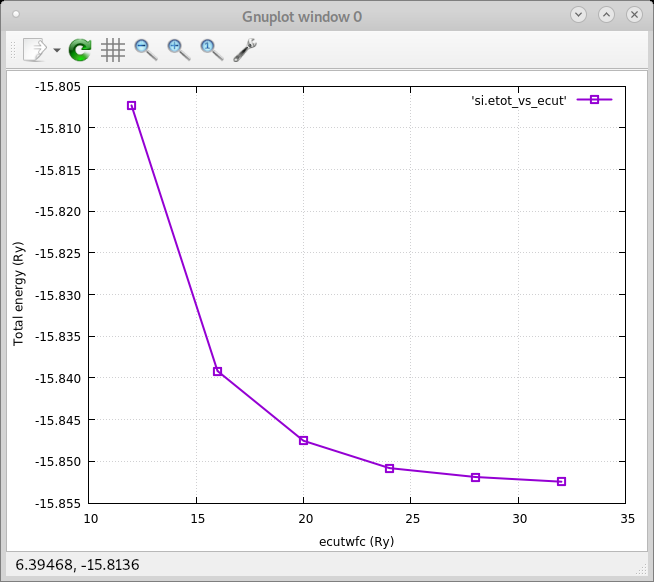
\includegraphics[width=11cm]{figs/ecut.png}
\end{flushright}

%%%%%%%%%%%%%%%%%%%%%%%%%%%%%%%%%%%%%%%%%%%%%%%%%%%%%%%%%%%%%
\head{1.1 Convergence w.r.t.\@{} the kinetic energy cutoff (IV)}
%
%\rightheader{\hspace{-0.8cm}
\includegraphics[width=3.4cm]{figs/QE.png}}

\begin{center}
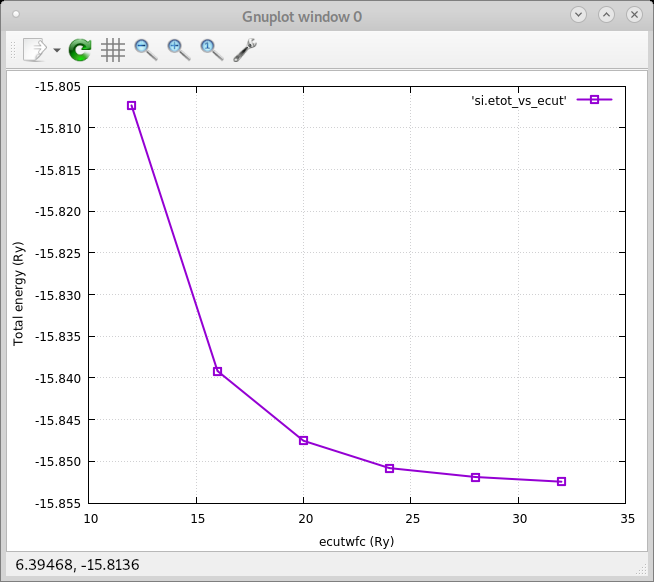
\includegraphics[width=10cm]{figs/ecut.png}
\end{center}
\vspace{-2cm}
{\burgundy Notes:}
\begin{itemize}
\item Convergence w.r.t.\@{} cutoff is a property of the {\em pseudopotential(s) used}.
\item 
Convergence of the {\em absolute energy} is typically slower than convergence of
{\em interesting physical properties}, e.g. structure.
\item 
Absolute values of total energy do not have any physical meaning 
(and depend upon the specific pseudopotential): only energy {\em
  differences} have meaning
\end{itemize}

%%%%%%%%%%%%%%%%%%%%%%%%%%%%%%%%%%%%%%%%%%%%%%%%%%%%%%%%%%%%%
\head{1.2 Convergence w.r.t.\@{} k-points}
\rightfooter{Example: \file{Day-2/example1.Si/ex2.kpoints/}}
\rightheader{\hspace{-0.8cm}
\includegraphics[width=4.5cm]{figs/QE.png}}

A sufficiently dense grid of k-points is needed in order to account
for {\em periodicity}.

To test the convergence w.r.t.\@{} k-points, you need to edit
the \card{K\_POINTS} card and request {\em automatic} Monkhorst-Pack
grids:
%
{\cardcolor
\begin{verbatim}
   K_POINTS automatic
   nk1 nk2 nk3   k1 k2 k3
\end{verbatim}
}
then step-wise increase \card{nk1=nk2=nk3} to, e.g., \card{2, 4, 6, 8}
(keep \card{k1=k2=k3=1}) and run \prog{pw.x} calculation for each
value of \card{nk1=nk2=nk3}.

For example, with PWTK this can be achieved with the following snippet:
{\codecolor
\begin{verbatim}
   load_fromPWI pw.si.scf.in

   foreach k {2 4 6 8} {
      K_POINTS automatic "$k $k $k  1 1 1"
      runPW pw.si.scf.$k.in
   }
\end{verbatim}
}

%%%%%%%%%%%%%%%%%%%%%%%%%%%%%%%%%%%%%%%%%%%%%%%%%%%%%%%%%%%%% 
\head{1.2 Convergence w.r.t.\@{} k-points (II)}
%
Description of the \card{K\_POINTS} card for {\em automatic} mode:
{\cardcolor
\begin{verbatim}
   K_POINTS automatic
   nk1 nk2 nk3   k1 k2 k3
\end{verbatim}
}

The first three \card{nk1 nk2 nk3} numbers mean {\em ``there are
  nk1,nk2,nk3 grid points along crystal axis 1,2,3''}; the second
three \card{k1 k2 k3} numbers, either 0 or 1, mean {\em ``grid starts
  from 0''} or {\em ''displaced by half a step''} along crystal axis
1,2,3\\

Also note that:
\begin{itemize}
\item  Convergence is not necessarily monotonic: 
  there is no variational principle w.r.t.\@{} number of k-points
\item {\gray The \card{2 2 2~~1 1 1} Monkhorst-Pack grid is the same as 
  the ``two Chadi-Cohen points'' {\small (see: D.J. Chadi and
M.L. Cohen, Phys. Rev. B {\bf 8}, 5747 (1973))}}
\end{itemize}

%%%%%%%%%%%%%%%%%%%%%%%%%%%%%%%%%%%%%%%%%%%%%%%%%%%%%%%%%%%%% 
\head{1.2 Convergence w.r.t.\@{} k-points (III)}
%
The PWTK script for testing the convergence with respect to k-points is
located in
\file{Day-2/example1.Si/ex2.kpoints/} directory (see \file{README.md}
for detailed instructions).

Within this directory execute:\\[0.5em]
\indent\prompt\code{pwtk kpoints.pwtk}\\[0.5em]
You should get a plot like this one:\\[-3cm]
\begin{flushright}
  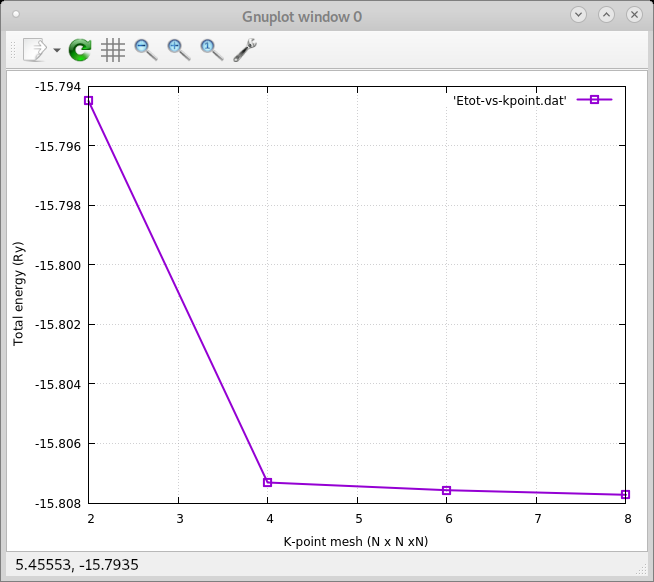
\includegraphics[width=12cm]{figs/etot-vs-kpoints.png}
\end{flushright}

%%%%%%%%%%%%%%%%%%%%%%%%%%%%%%%%%%%%%%%%%%%%%%%%%%%%%%%%%%%%%
\head{1.3 Equation of State: silicon}
\rightfooter{Example: \file{Day-2/example1.Si/ex3.alat/}}
%
Equilibrium in Si is determined by the minimum-energy lattice
parameter alone: there are no forces on atoms due to symmetry (you can
verify this by setting \var{tprnfor=.true.} in namelist
\nml{\&CONTROL} and looking for forces reprinted at the end).

To find the lattice parameter:
\begin{itemize}
\item Choose suitable values for \var{ecutwfc} and k-point 
grid {\small (e.g. \var{30} Ry and \var{4 4 4~~1 1 1})}
\item Run \prog{pw.x} for values of \var{celldm(1)} ranging from
  9.7 to 10.7 in steps of 0.1 a.u.
\end{itemize}

With PWTK this can be achieved with the following snippet:
{\codecolor
\begin{verbatim}
   load_fromPWI pw.si.scf.in

   foreach alat [seq 9.7 0.1 10.7] {
      SYSTEM "celldm(1) = $alat"
      runPW pw.si.scf.$alat.in
   }
\end{verbatim}
}

%%%%%%%%%%%%%%%%%%%%%%%%%%%%%%%%%%%%%%%%%%%%%%%%%%%%%%%%%%%%% 
\head{1.3 Equation of State: silicon (II)}

The corresponding PWTK script is located in
\file{Day-2/example1.Si/ex3.alat/} directory (see \file{README.md} for
detailed instructions).

\parbox{0.5\textwidth}{
  Within this directory execute:\\[0.5em]
  \indent\prompt\code{pwtk alat.pwtk}\\[0.5em]

  The experimental lattice parameter for Si is 5.47 \AA\ or 10.26
  a.u..  This is a case where plain simple LDA yields remarkable results.\\
  You may experiment changing cutoff, k-points, pseudopotential,
  ...\\[0.5em]
  You should find that:
} \parbox{0.5\textwidth}{
  \begin{flushright}
    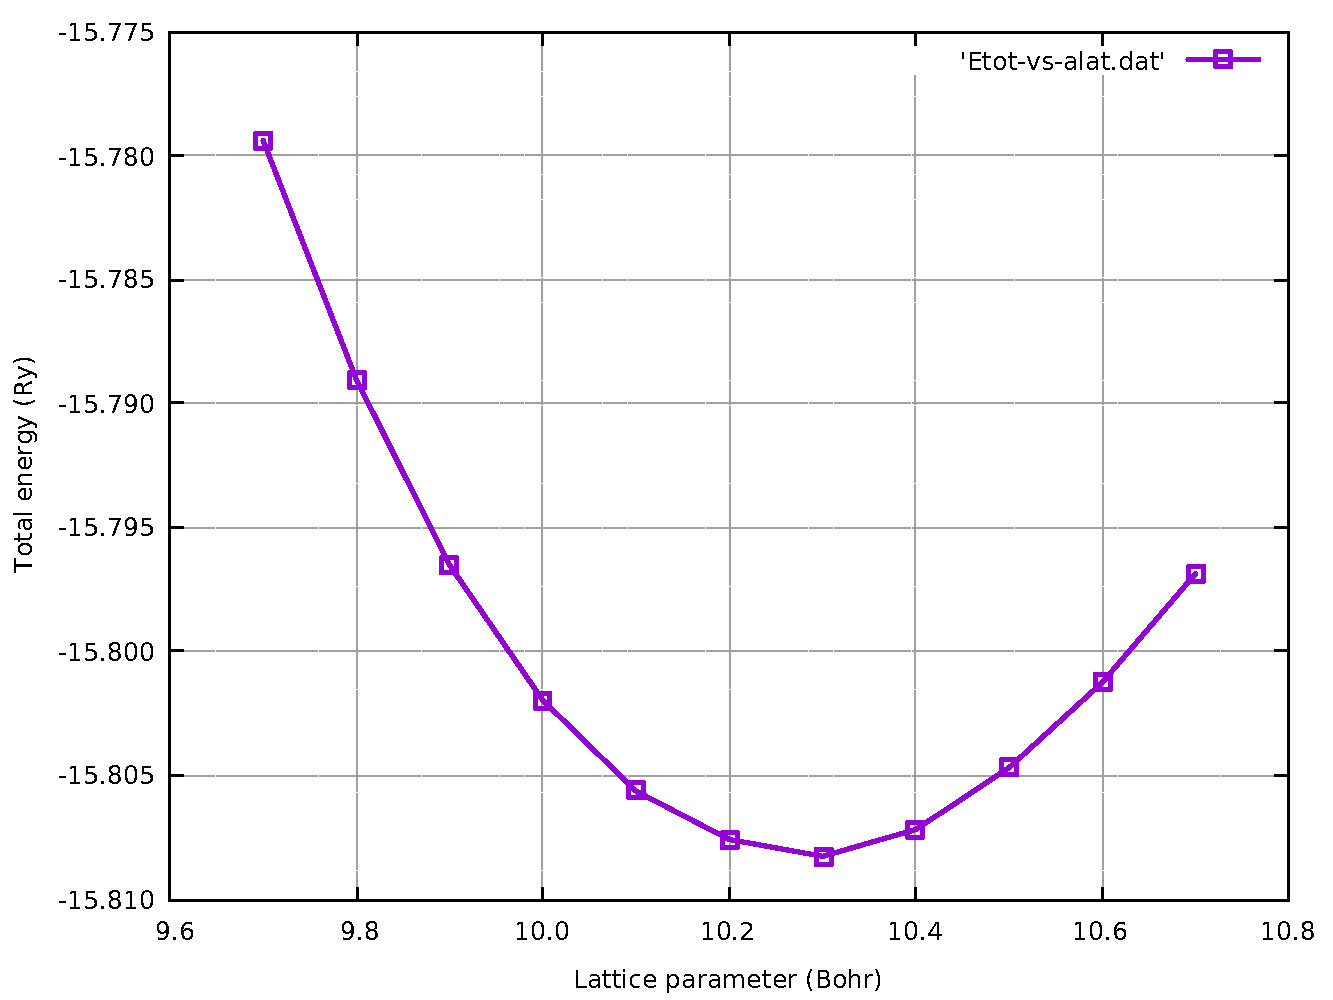
\includegraphics[width=0.45\textwidth]{figs/etot-vs-alat.pdf}
  \end{flushright}
}
\begin{itemize}
\item The energy vs lattice parameter $E(a)$ curves are shifted down rather 
  uniformly with increasing cutoff and are not strongly dependent on k-points.
\item Structural properties and energy differences converge faster than total
  energies.
\end{itemize}

%%%%%%%%%%%%%%%%%%%%%%%%%%%%%%%%%%%%%%%%%%%%%%%%%%%%%%%%%%%%% 
\head{1.3 Equation of State: silicon (III)}
%
Use the code \prog{ev.x} to fit your results to a
phenomenological equation-of-state (EOS, e.g. Murnaghan) and to get
accurate values for the lattice parameter and for the bulk modulus.

The \prog{ev.x} code prompts for some data and reads a data-file like
the one produced by the \file{alat.pwtk} script (the data-file is
\file{Etot-vs-alat.dat}). For cubic systems a data-file should contain
the following rows:
\begin{quote}
$a_1\qquad E(a_1)$\\
$a_2\qquad E(a_2)$\\
$a_3\qquad E(a_3)$\\
...\\  
\end{quote}


%%%%%%%%%%%%%%%%%%%%%%%%%%%%%%%%%%%%%%%%%%%%%%%%%%%%%%%%%%%%%
\head{1.4 Band Structure of Silicon}
\rightfooter{Example: \file{Day-2/example1.Si/ex4.bands/}}
%
The scheme to calculate the bands (spaghetti plot) is the following:
\parbox{0.7\textwidth}{
  \begin{enumerate}
  \item SCF \prog{pw.x} calculation (\var{calculation = 'scf'})
  \item ``bands''-type non-SCF \prog{pw.x} calculation
    (fixed-potential) with:
    \begin{itemize}
    \item \var{calculation = 'bands'}
    \item the number of Kohn-Sham states explicitly set (variable
      \var{nbnd})
    \item a suitable path of k-points specified in \card{K\_POINTS} (in
      this example we use the $L-\Gamma-X-W-K-L$ path)
    \end{itemize}
  \item \prog{bands.x} calculation, which, among others, produces
    data-files for the spaghetti plot
  \end{enumerate}
}\parbox{0.3\textwidth}{
 \begin{flushright}
    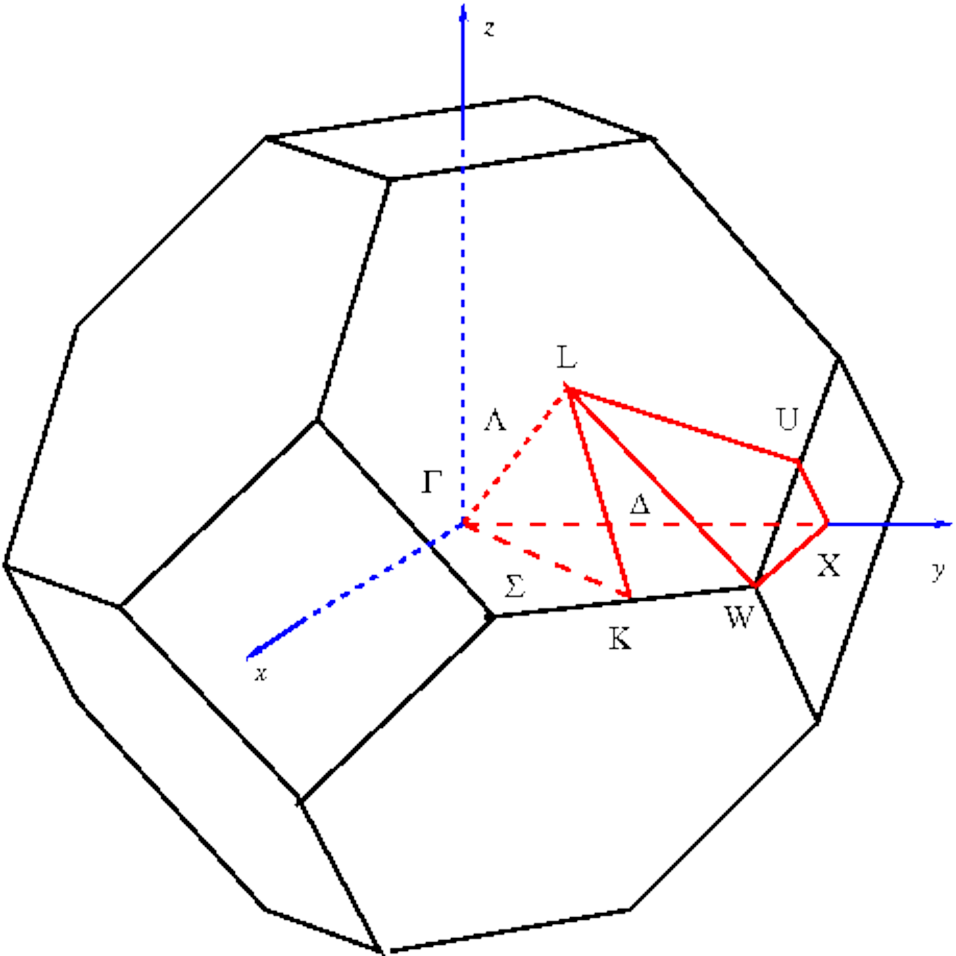
\includegraphics[width=0.27\textwidth]{figs/fcc_brillouin.pdf}
  \end{flushright}
}

{\em Important:} \var{outdir} and \var{prefix} must be the same for
``bands'' and ``scf'' \prog{pw.x} calculations and for
the \prog{bands.x} calculation\\
{\em Important:} the k-point path must be continuous in k-space

%%%%%%%%%%%%%%%%%%%%%%%%%%%%%%%%%%%%%%%%%%%%%%%%%%%%%%%%%%%%% 
\head{1.4 Band Structure of Silicon (II)}
%
The input for the \prog{bands.x} program is the following:
{\codecolor
\begin{verbatim}
&BANDS
   prefix='...', outdir='...', filband = 'Si.bands.dat', lsym=.true.
/
\end{verbatim}
}
%
Two files are produced: \file{Si.bands.dat.gnu}, directly plottable
with \prog{gnuplot}, and \file{Si.bands.dat}, for further processing
by the auxiliary command \prog{plotband.x}.

If option \var{lsym=.true.}, \prog{bands.x} performs a symmetry
analysis. An additional file \file{Si.bands.dat.rep} is generated,
containing information on symmetry labels of the various bands.

The snippet for running all three calculations manually is:\\[0.5em]
\exec{pw.x -in pw.Si.scf.in > pw.Si.scf.out}\\
\exec{pw.x -in pw.Si.bands.in > pw.Si.bands.out}\\
\exec{bands.x -in bands.Si.in > bands.Si.scf.out}\\[0.5em]
{\bf  but} we will use a PWTK script instead.

%%%%%%%%%%%%%%%%%%%%%%%%%%%%%%%%%%%%%%%%%%%%%%%%%%%%%%%%%%%%% 
\head{1.4 Band Structure of Silicon (III)}
%
To execute the PWTK script that will perform all the needed
calculations for plotting the bands, proceed as follows:\\
\parbox{0.65\textwidth}{
  \begin{itemize}
  \item move to directory\\
    \file{Day-2/example1.Si/ex4.bands/} and read the \file{README.md} file
  \item set suitable values for \var{celldm(1)}, \var{ecutwfc}, and
    \card{K\_POINTS}
  \item and execute: ~\code{pwtk bands.pwtk}
  \item you may set the \var{Efermi} value to the top of the occupied
    bands in the gnuplot file \file{plot.gp} (see the instructions in
    \file{README.md}); then re-plot spaghetti with: \code{gnuplot
      plot.gp}
  \end{itemize}
}\parbox{0.35\textwidth}{
  \begin{flushright}
    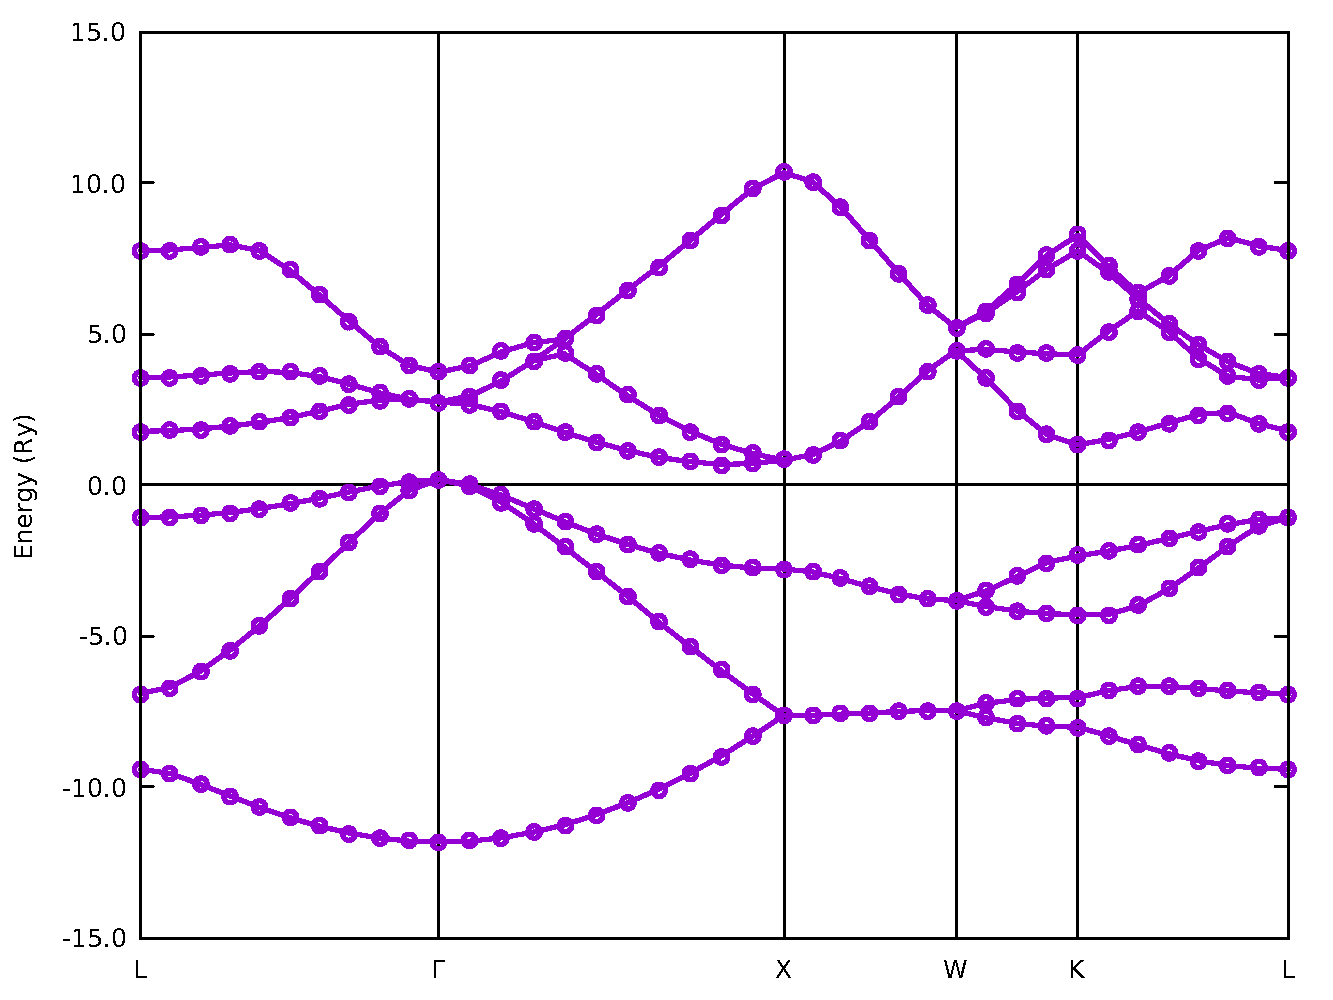
\includegraphics[width=0.35\textwidth]{figs/si-bands.pdf}
  \end{flushright}
}

{\em Remark:} in PWTK, once \var{outdir} and \var{prefix} are set,
they are automatically inherited for subsequent calculations.

%%%%%%%%%%%%%%%%%%%%%%%%%%%%%%%%%%%%%%%%%%%%%%%%%%%%%%%%%%%%%
\head{Auxiliary program plotband.x} 
\prog{plotband.x} prompts for terminal input:
{\codecolor
\begin{verbatim}
• plotband.x 
Input file > Si.bands.dat
Reading    8 bands at     39 k-points
Range:   -5.6940   16.4680eV  Emin, Emax > -5.6940   16.4680
high-symmetry point: -0.5000 0.5000 0.5000   x coordinate   0.0000
high-symmetry point:  0.0000 0.0000 0.0000   x coordinate   0.8660
high-symmetry point:  0.0000 0.0000 1.0000   x coordinate   1.8660
high-symmetry point:  0.0000 0.5000 1.0000   x coordinate   2.3660
high-symmetry point:  0.0000 0.7500 0.7500   x coordinate   2.7196
high-symmetry point: -0.5000 0.5000 0.5000   x coordinate   3.3320
output file (gnuplot/xmgr) > Si.bands.plot   
bands in gnuplot/xmgr format written to file Si.bands.plot
output file (ps) > (press Return)
\end{verbatim}
}
%
If symmetry analysis was performed in the previous step, the output is
written to several plottable files \file{Si.bands.plot.{\em N.M}},
where $N$ labels the high-symmetry lines,
$M$ labels irreducible representations.

%%%%%%%%%%%%%%%%%%%%%%%%%%%%%%%%%%%%%%%%%%%%%%%%%%%%%%%%%%%%%
\head{2. A metallic example: Aluminum}
\rightfooter{Example: \file{Day-2/example2.Al/}}

%
Aluminum is even simpler than Silicon: one atom per unit cell
in an fcc lattice.\\
{\bf\burgundy BUT:} it is a metal, only valence bands and a few k-points will
not suffice.
\begin{itemize}
\item move to the \file{Day-2/example2.Al/} directory
\item read the \prog{pw.x} input file \file{pw.al.scf.in}
\item notice the presence of new variables: \var{occupations},
\var{smearing}, \var{degauss};
\item run \prog{pw.x} as:\\[0.5em]
  \exec{pw.x -in pw.al.scf.in > pw.al.scf.out}
\item in the output file notice that
  \begin{itemize}
  \item the number of bands (Kohn-Sham states)
    is automatically set to a value larger than the number of
    electrons divided by 2
  \item the Fermi energy is computed.
  \end{itemize}
\end{itemize}

%%%%%%%%%%%%%%%%%%%%%%%%%%%%%%%%%%%%%%%%%%%%%%%%%%%%%%%%%%%%%
\head{2.1 Convergence with respect to k-points, degauss, and smearing} 
\rightfooter{Example: \file{Day-2/example2.Al/ex1.degauss/}}
\rightheader{}
%
This is a {\it ``three-dimensional''} convergence test, where the
number of k-points and values of \var{degauss} and \var{smearing}
variables are varied. In particular, we will vary:
\begin{enumerate}
\item[]
  \begin{itemize}
  \item \var{smearing} variable, possible values:
    \flag{'gauss'} (or \flag{'g'}), \flag{'marzari-vanderbilt'} (or
    \flag{'m-v'}), \flag{'methfessel-paxton'} (or \flag{'m-p'})
  \item \var{degauss} variable, in range from 0.003 to 0.1
  \item k-points using the {\em automatic} grids of \card{4 4 4},
    ~\card{8 8 8}, ~\card{12 12 12}, and \card{16 16 16}    
  \end{itemize}
\end{enumerate}
With PWTK this can be achieved with the following snippet:
{\codecolor\small
\begin{verbatim}
    foreach nk {4 8 12 16} {
        foreach smear {'gauss'  'm-p'  'm-v'} {
            foreach degauss {0.003 0.01 0.03 0.1} {
                SYSTEM " smearing = $smear  
                         degauss  = $degauss "
                K_POINTS automatic "$nk $nk $nk   1 1 1"
                runPW pw.Al.scf.$nk.$smear.$degauss.in
            }
        }
    }
\end{verbatim}
}

%%%%%%%%%%%%%%%%%%%%%%%%%%%%%%%%%%%%%%%%%%%%%%%%%%%%%%%%%%%%% 
\head{2.1 Convergence with respect to k-points, degauss, and smearing} 
%
\begin{itemize}
\item move to \file{Day-2/example2.Al/ex1.degauss/} directory
\item execute: ~\code{pwtk degauss.pwtk} 
\end{itemize}
\vspace{-1em}
Notice how much slower the convergence is for metals than for insulators!

Both \flag{m-v} and \flag{m-p} depend much less upon \var{degauss} and
allow for faster and safer convergence than simple Gaussian
broadening. For Al and \flag{m-v} or \flag{m-p} smearing, good
convergence is achieved for a \card{12 12 12} k-point grid and
\var{degauss} $\sim 0.01$ to $0.05$ Ry.\\[1em]
\centerline{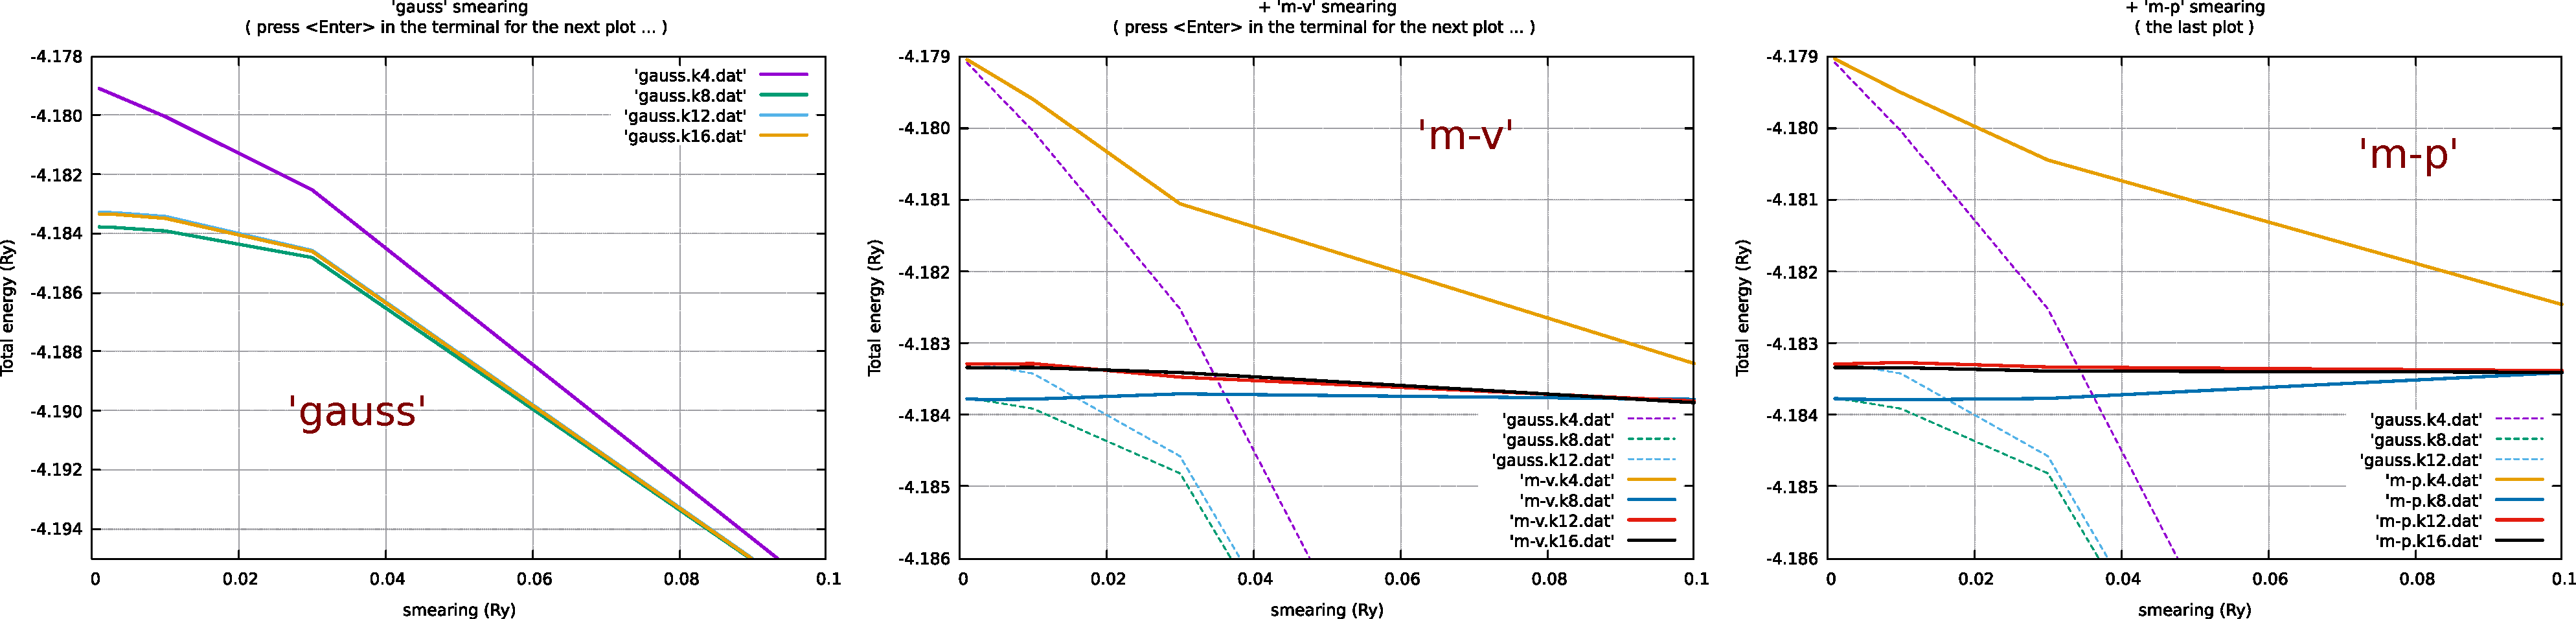
\includegraphics[width=1.0\textwidth]{figs/smearing.pdf}}
{\small\gray Beware that you cannot reduce the broadening too much:
  the energy levels must have some overlap, or else the advantage of
  broadening is lost!}


%%%%%%%%%%%%%%%%%%%%%%%%%%%%%%%%%%%%%%%%%%%%%%%%%%%%%%%%%%%%% 
\head{2.2 How to plot charge-density}
\rightfooter{Example: \file{Day-2/example2.Al/ex2.chdens/}}
\rightheader{\hspace{-0.8cm}
\includegraphics[width=4.5cm]{figs/QE.png}}
%
Example \file{Day-2/example2.Al/ex2.chdens/} shows how to calculate the
valence and the all electron charge density (the latter requires a PAW
potential and a very large cutoff energy)
\begin{itemize}
\item move to \file{Day-2/example2.Al/ex2.chdens/} directory ({\it
    chdens} is an acronym for charge-density)
\item execute: ~\code{pwtk 1-chdens.pwtk}\\
  this script calculates and ``plots'' the valence charge density;
  notice that the electron charge is located mainly in interstitial
  regions (due to the use of a pseudo-potential, there is {\it almost
    no} charge in close vicinity of nuclei; see the next page)
\item the scheme to calculate and plot the charge-density is:
  \begin{enumerate}
  \item make an SCF \prog{pw.x} calculation
  \item make a post-processing \prog{pp.x} calculation
    (\var{plot\_num=0} for charge density) and instruct the program to
    write charge density in a suitable format
  \item plot the charge density by \prog{xcrysden} (let's plot density
    in contour/colorplane style; follow the instructions of tutor and
    select density range from \code{0.0} to \code{0.05})
  \end{enumerate}
\end{itemize}

%%%%%%%%%%%%%%%%%%%%%%%%%%%%%%%%%%%%%%%%%%%%%%%%%%%%%%%%%%%%% 
\head{2.2 How to plot charge-density (II)}

\begin{itemize}
\item to calculate all-electron {\bf valence} and {\bf total} charge densities,
  execute:\\[0.5em]
  \exec{pwtk 2-chdens-paw.pwtk}\\[0.5em]
  (note that \var{plot\_num=17} for all-electron valence density and
  \var{plot\_num=21} for all-electron total density)

\item comparison between pseudopotential (PP) valence-density vs.\@{} all-electron densities
  (valence and total):
\end{itemize}
\centerline{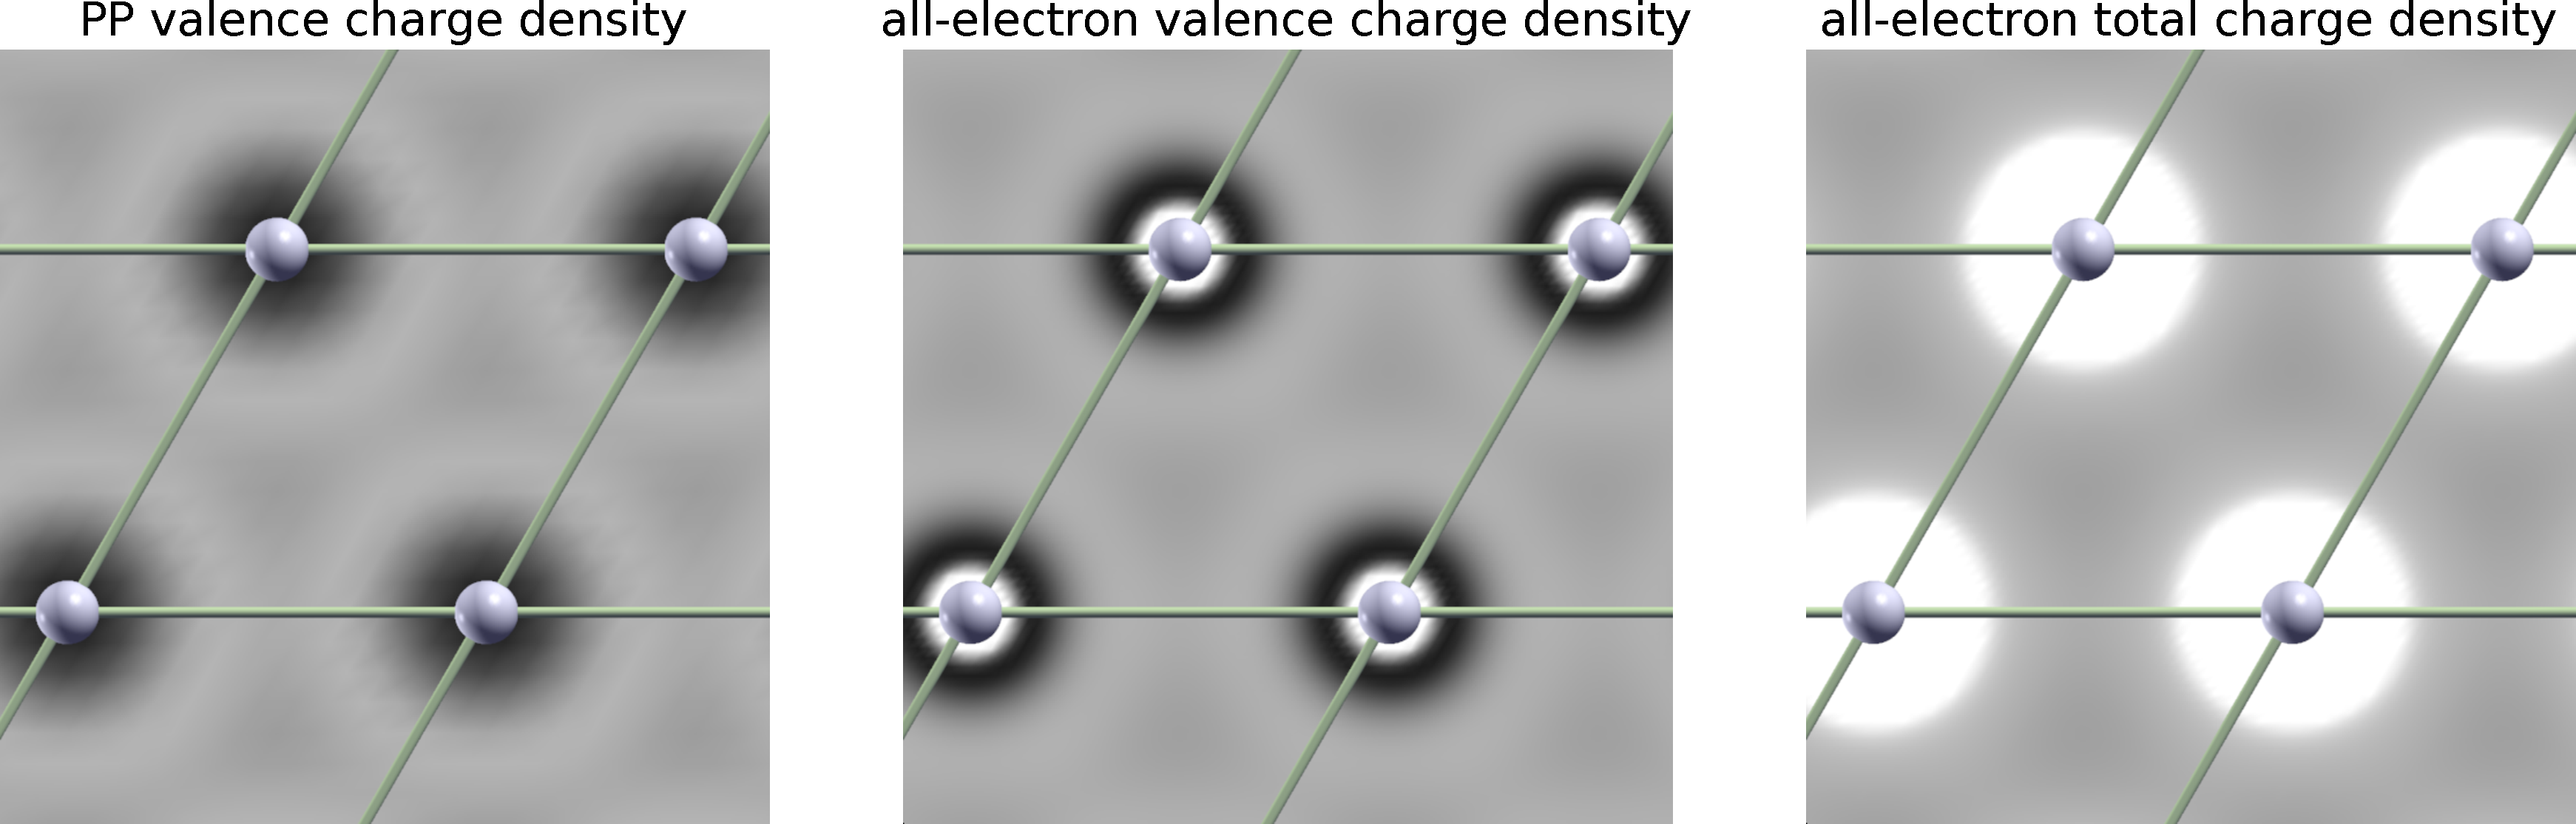
\includegraphics[width=1.0\textwidth]{figs/Al-chdens.pdf}}

%%%%%%%%%%%%%%%%%%%%%%%%%%%%%%%%%%%%%%%%%%%%%%%%%%%%%%%%%%%%% 
\head{3. A magnetic example: Iron bulk}
\rightfooter{Example: \file{Day-2/example3.Fe/}}
%
Fe has two remarkable features: it is magnetic and it ``calls for'' an
Ultrasoft PP (USPP) since its localized 3d atomic states are very
hard.
\begin{itemize}
\item move to the \file{Day-2/example3.Fe/} directory and read the
  \prog{pw.x} input file \file{pw.fe\_fm.scf.in}
\item the structure is bcc (\var{ibrav=3}) with one atom per unit cell
\item notice (i) variables \var{nspin} and of
  \var{starting\_magnetization}, indicating spin-polarized calculation
  (\var{nspin=2}) with unconstrained total magnetization with only the
  initial guess for the magnetization given and (ii) variables for
  {\em metallic} system (\var{occupations}, \var{smearing},
  \var{degauss})
\item notice that this calculation uses GGA (PBE): it is specified
inside the PP file (can be guessed from the PP file name),
reprinted on output as "Exchange-correlation"
\item also notice that with USPP, it is typically needed to set
\var{ecutrho $ > 4 * $ecutwfc}
(it should be at least 8 to 12 times larger)
\end{itemize}

%%%%%%%%%%%%%%%%%%%%%%%%%%%%%%%%%%%%%%%%%%%%%%%%%%%%%%%%%%%%% 
\head{3. Magnetic structures}
%
Run \prog{pw.x} in the usual way (\code{pw.x -in
  pw.fe\_fm.scf.in > pw.fe\_fm.scf.out}). In the output, notice:
\begin{itemize}
\item the number of k-points is doubled w.r.t the non-magnetic case:
  the first set of k-points contains spin-up states, the second set
  spin-down states\\
  {\small (use \var{verbosity='high'} in namelist \nml{\&CONTROL} if
    there are more than 100 k-points)}
\item in the output notice such lines:
  {\codecolor
\begin{verbatim}
     total magnetization       =     2.41 Bohr mag/cell
     absolute magnetization    =     2.60 Bohr mag/cell
\end{verbatim}
  }
  %
  Since there is a single (magnetic) atom per unit cell, the only
  possible magnetic structure is ferromagnetic.
\end{itemize}

%%%%%%%%%%%%%%%%%%%%%%%%%%%%%%%%%%%%%%%%%%%%%%%%%%%%%%%%%%%%% 
\head{3. Magnetic structures: going antiferromagnetic}
\rightheader{\hspace{-0.8cm}
\includegraphics[width=3.4cm]{figs/QE.png}}

\begin{itemize}
  \item To reach antiferromagnetic states, you need to:
  \begin{itemize}
  \item introduce a {\burgundy supercell} with two sublattices of 
    different species of atoms (even if they are the same,
    it is important that they are labeled as different)
  \item start with opposite initial magnetization for the two 
    sublattices
  \end{itemize} 

\item Can you write input data for an AFM structure?\\
  {\gray\small {\bf hint:} split bcc into two simple cubic sublattices,
    \var{ibrav=1}, with two atoms at (0,0,0) and
    $(\frac{1}{2},\frac{1}{2},\frac{1}{2})$}.
\end{itemize}

\vfill

As a convenience, an antiferromagnetic file is provided
(\file{pw.fe\_afm.scf.in})

You can compare the ferromagnetic and antiferromagnetic files
by:\\[1em]
\exec{diff pw.fe\_fm.scf.in pw.fe\_afm.scf.in}



%%%%%%%%%%%%%%%%%%%%%%%%%%%%%%%%%%%%%%%%%%%%%%%%%%%%%%%%%%%%%
\head{3.1 Convergence tests for ultrasoft pseudopotential(s)}
\rightfooter{Example: \file{Day-2/example3.Fe/ex1.ecut/}}
\rightheader{}%\hspace{-0.8cm}
\includegraphics[width=3.4cm]{figs/QE.png}}

%
For computational efficiency, it is convenient to keep \var{ecutwfc}
as low as possible, while \var{ecutrho} is less critical
{\gray\small (look at 
the CPU time report at the end of an output: there are very many
\texttt{fft{\bf w}}, depending upon \var{ecutwfc}, while a much smaller
number of \texttt{fft} depends upon \var{ecutrho})}

Set the \var{ecutrho/ecutwfc} ratio ($dual$) to 4, 8, 12 and compute
the energy vs \var{ecutwfc} curve. For $dual=4$ it will look funny:
energy {\em increases} with increasing cutoff (see next page), but for
a higher $dual$ (i.e.\@{} better description of augmentation charge) the
normal behavior is observed.
%\parbox{12cm}{
%\centerline{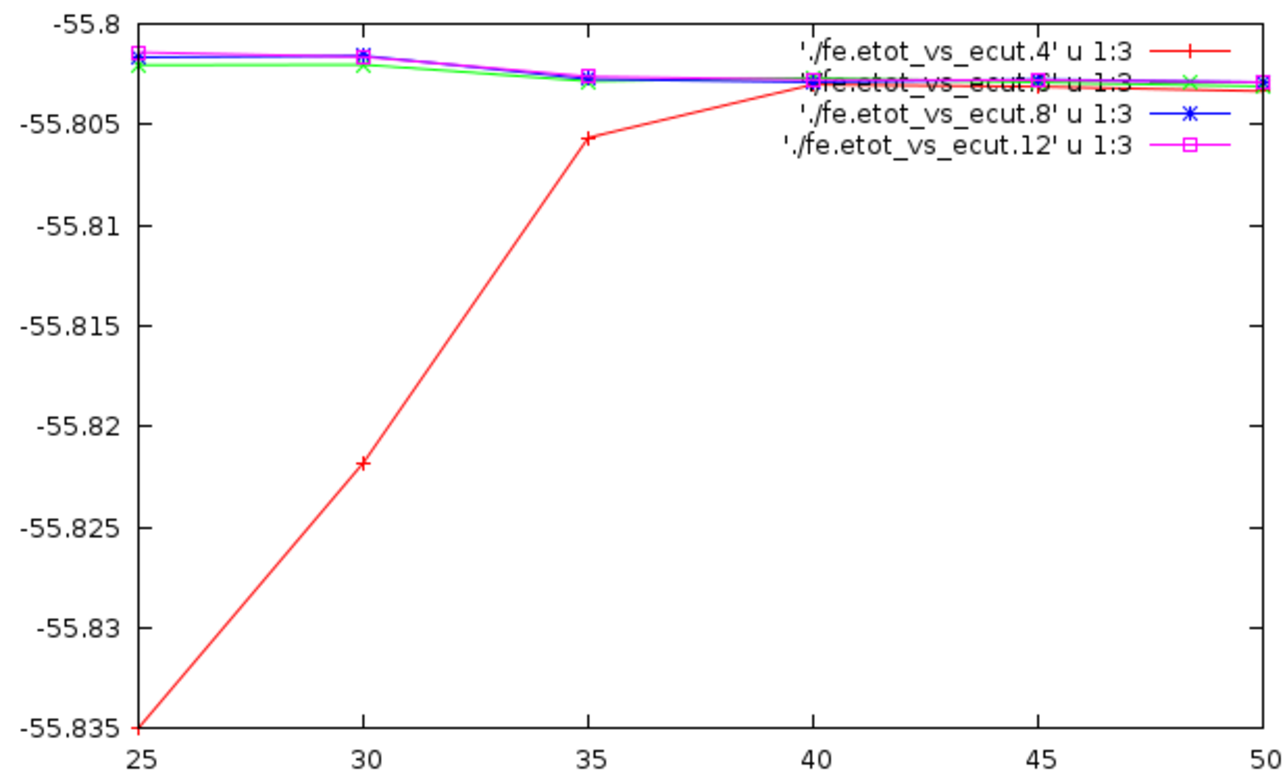
\includegraphics[width=10cm]{figs/fe-ecut.pdf}}
%}

The corresponding PWTK snippet is:
{\codecolor\small
\begin{verbatim}
   load_fromPWI pw.fe_fm.scf.in

   foreach dual {4 8 12} {
      foreach ecut {25 30 35 40 45 50} {
         SYSTEM "ecutwfc = $ecut
                 ecutrho = $ecut*$dual "
         runPW pw.fe_fm.scf.$dual.$ecut.in
      }
   }
\end{verbatim}
}

%%%%%%%%%%%%%%%%%%%%%%%%%%%%%%%%%%%%%%%%%%%%%%%%%%%%%%%%%%%%% 
\head{3.1 Convergence tests for ultrasoft pseudopotential(s)}
%\head{Convergence check for USPP (II)}

A PWTK script to make convergence check for USPP is provided, i.e.:

\parbox{0.55\textwidth}{
\begin{itemize}
\item move to directory:\\ \file{Day-2/example3.Fe/ex1.ecut/}
\item execute: ~\code{pwtk ecut.pwtk}
\item you should obtain such a plot\\
  {\small (notice that curves for $dual=8$ and $12$\\almost coincide)}
\end{itemize}
}\parbox{0.45\textwidth}{
  \begin{flushright}
    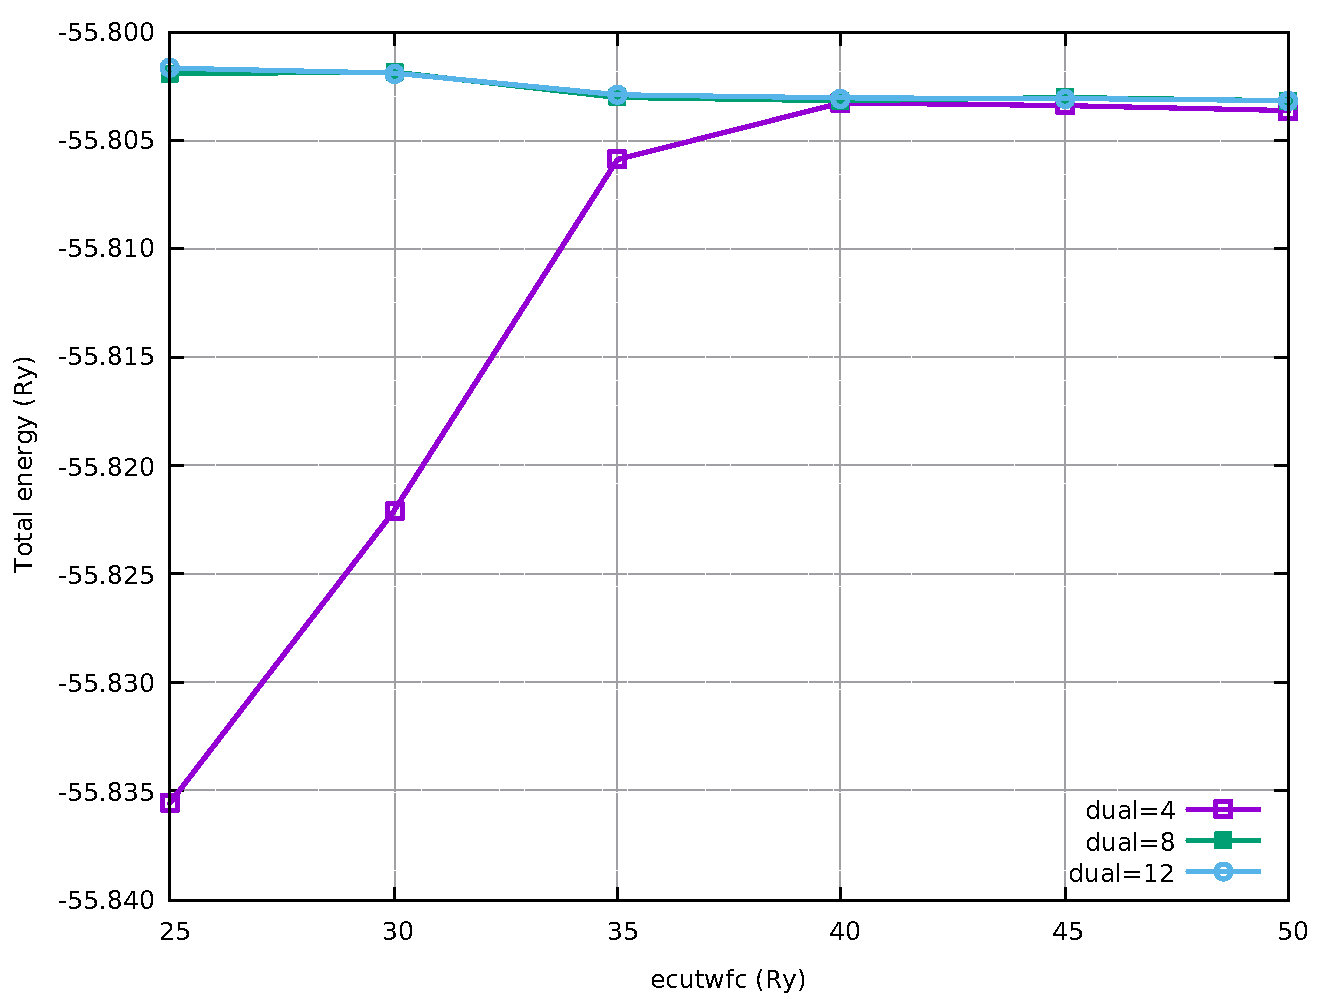
\includegraphics[width=0.45\textwidth]{figs/fe-dual+k-points.pdf}
  \end{flushright}
}
\vfill
{\bf Homework:} for converged values of both cutoffs and k-points, you may
  compare the stability of iron in the bcc, fcc, hcp
  phases (the latter being a slightly more complicated structure)

%%%%%%%%%%%%%%%%%%%%%%%%%%%%%%%%%%%%%%%%%%%%%%%%%%%%%%%%%%%%%
\head{3.2 Density of States (DOS) and Projected DOS (PDOS)}
\rightfooter{Example: \file{Day-2/example3.Fe/ex2.dos/}}
\rightheader{}

%
\begin{enumerate}
\item move to \file{Day-2/example3.Fe/ex2.dos/} directory and
\item edit the \file{dos.pwtk} script and set \var{ecutwfc} and
  \var{ecutrho} to appropriate values
\item execute: ~\code{pwtk dos.pwtk}\\
  {\small (this script calculates both total DOS and DOS projected (PDOS) to
  atomic orbitals)}
\end{enumerate}
\centerline{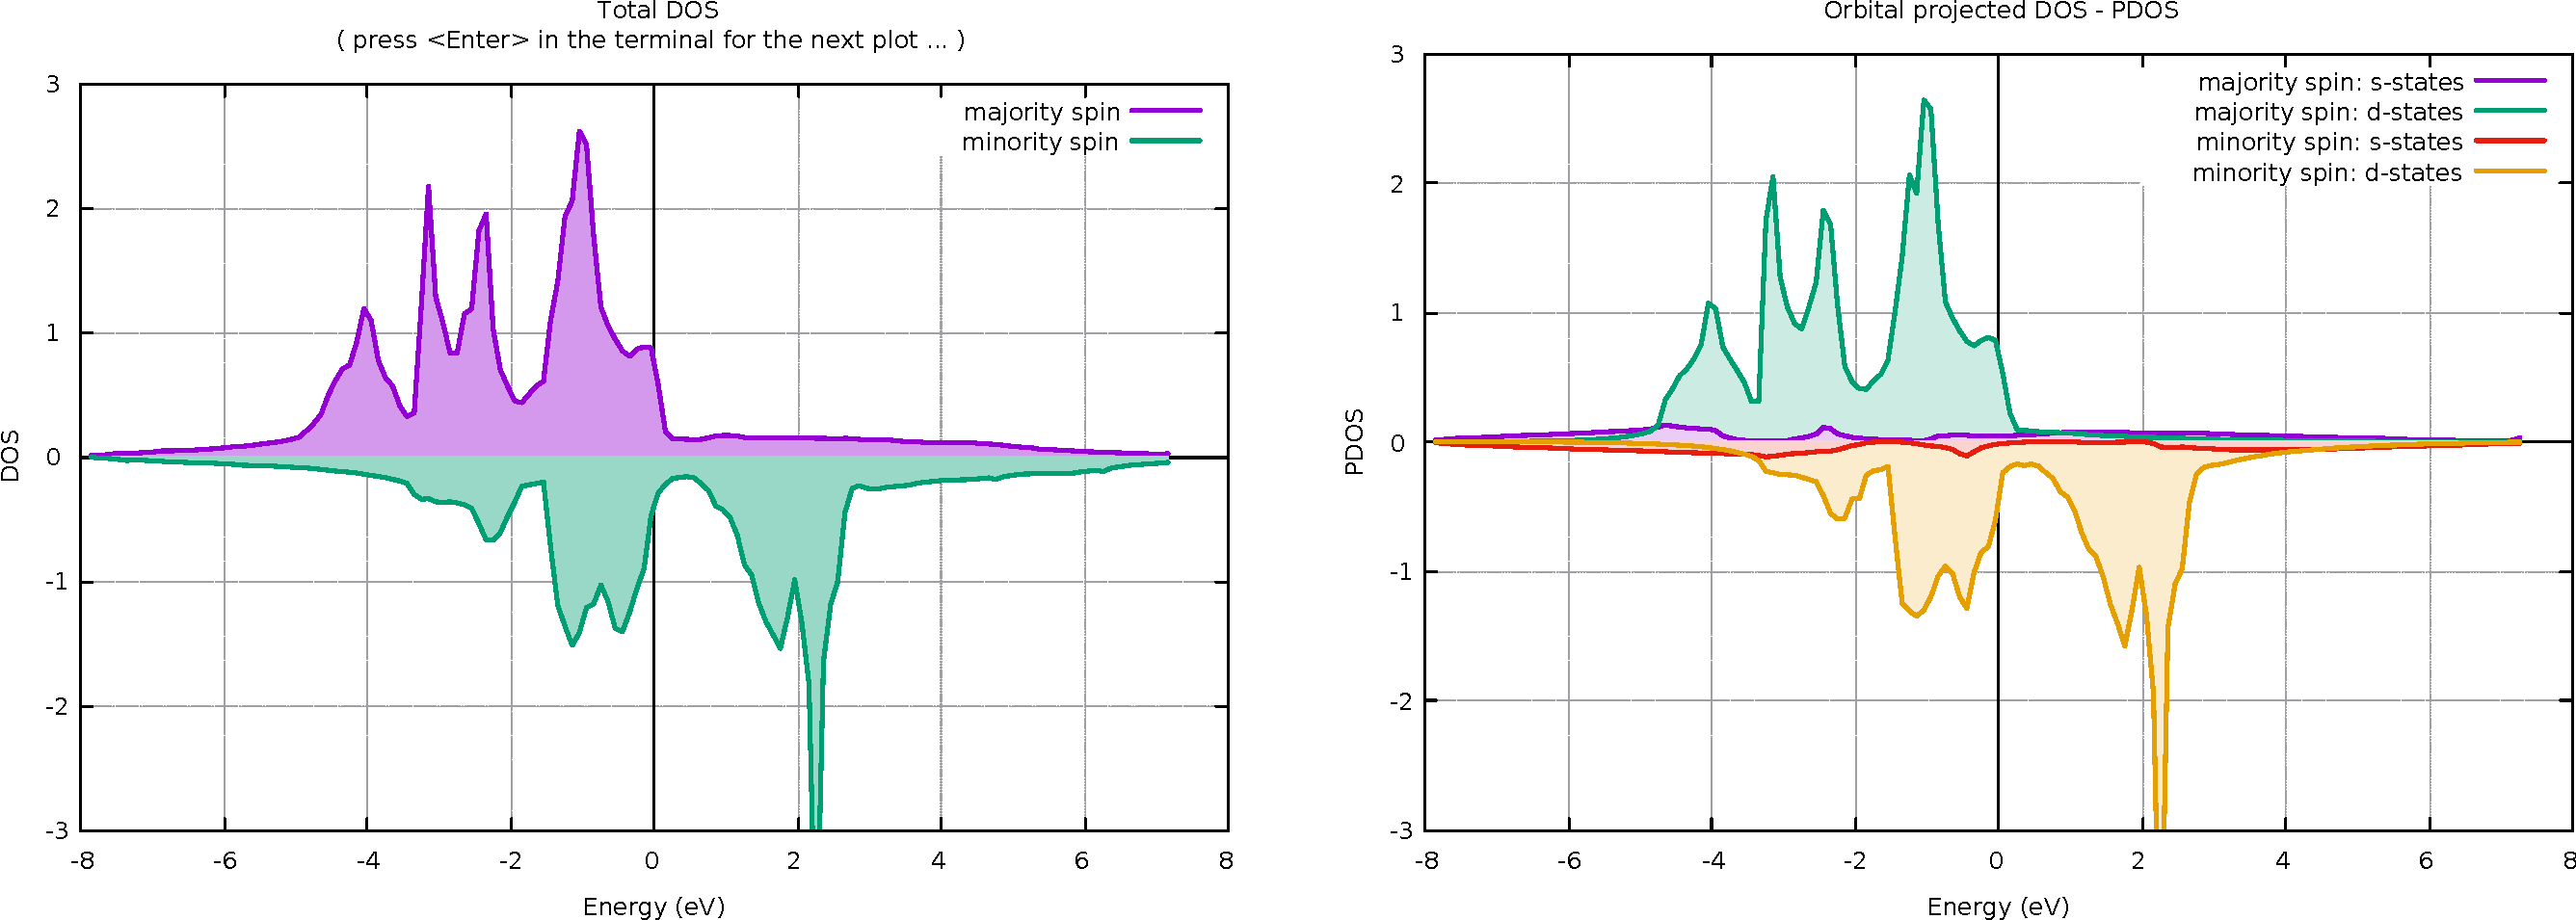
\includegraphics[width=1.0\textwidth]{figs/fe-dos+pdos.pdf}}

%%%%%%%%%%%%%%%%%%%%%%%%%%%%%%%%%%%%%%%%%%%%%%%%%%%%%%%%%%%%%
\head{3.2 Density of States (DOS) and Projected DOS (PDOS)}
The scheme to calculate DOS and PDOS consists of:\vspace{-0.8em}
\begin{enumerate}
\item an SCF \prog{pw.x} calculation (\var{calculation='scf'})\vspace{-0.8em}
\item a non-SCF \prog{pw.x} calculation (\var{calculation='nscf'}),
  where:\vspace{-0.3em}
  \begin{itemize}
  \item the same \var{prefix} and \var{outdir} are used as in the preceding SCF calculation
  \item a denser k-point mesh is specified
  \item in this example the {\em linear tetrahedron method} is used\\
    (variable \var{occupations='tetrahedra'})
  \end{itemize}\vspace{-0.8em}
\item a \prog{dos.x} calculation to calculate DOS {\small\gray (DOS is
    written to a file as specified by the \var{fildos} variable in the
    \prog{dos.x} input; also here the values of \var{prefix} and
    \var{outdir} are the same as for SCF \prog{pw.x}
    calculation)}\vspace{-0.8em}
\item a \prog{projwfc.x} calculation to calculate PDOS projected to
  atomic states {\small\gray (this calculation is analogous to
    \prog{dos.x} one,
    inputs are also very similar; you can compare them as:}\\[0.5em]
  \exec{diff dos.Fe.in projwfc.Fe.in}\\[0.5em]
  {\small\gray the difference is that \prog{dos.x} uses the \var{fildos}
    whereas \prog{projwfc.x} uses the \var{filpdos} variable)}
\end{enumerate}
Explore the content of \var{fildos} and \var{filpdos} files!  
\end{document}

%%% Local Variables:
%%% mode: latex
%%% TeX-master: t
%%% End:
